\section{Evaluación 4.- Configuración de Servicios}
\subsection{Servidor de información HTTP}
\noindent
El servidor HTTP, fue implementado usando Python a través de una librería para el desarrollo web y de apis llamada Flask, esto nos permite tener un servidor multiplataforma, por lo cual no está limítado a correr bajo ciertos entornos. Esto es bueno al momento de realizar pruebas, como es nuestro caso.\\ Para ejecutar el servidor, basta con tener python 3 y flask instalados. Además de que Flask permite trabajar con certificados ssl en caso de ser necesario, además de que permite recibir conexiones desde otros equipos de cómputo conectados a la red.\\ Para probar la funcionalidad del server, se ejecutó en un equipo, y posteriormente usando la utilidad httpie, se realizó una petición get al mismo desde otro equipo, el cual en este caso era una máquina virtual. El resultado de la petición se puede observar en la Figura \ref{fig:http1}.
\begin{figure}[H]
  \centering
    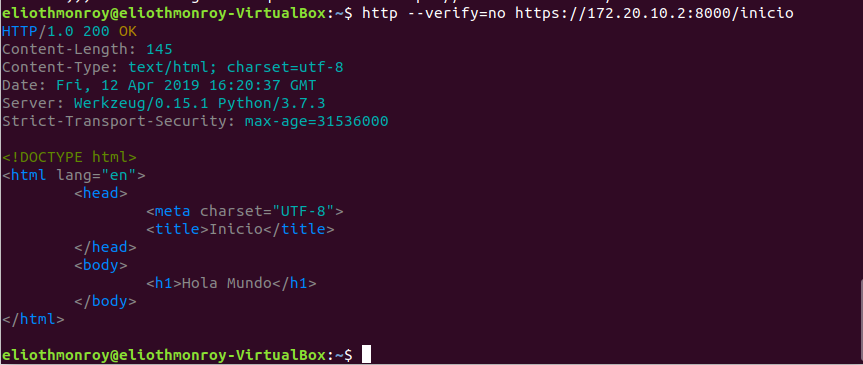
\includegraphics[scale=.54]{imagenes/primero/httpscreenshot.png}
    \caption{Funcionamiento correcto de servidor de información HTTP}
    \label{fig:http1}
\end{figure}
\subsection{Servicio de Acceso Seguro SSH (Secure Shell)}
\noindent
Para el funcionamiento del servicio de SSH se necesita un cliente y un servidor; el Servidor SSH fue implementado en Ubuntu.
\subsubsection{Implementación del Servidor SSH}
\begin{enumerate}
    \item Ejecutar los siguientes comandos en una Terminal de Linux:\\
     \\sudo apt-get update\\
     sudo apt install openssh-server\\
     \begin{figure}[H]
  \centering
    
\includegraphics[scale=1]{imagenes/primero/1.png}
    \caption{Instalación del Servidor de SSH}
    \label{fig:http1}
\end{figure}
    \item para revisar el status del servicio se ejecuta la linea de comando\\
         sudo systemctl status ssh \\
         \begin{figure}[H]
  \centering
    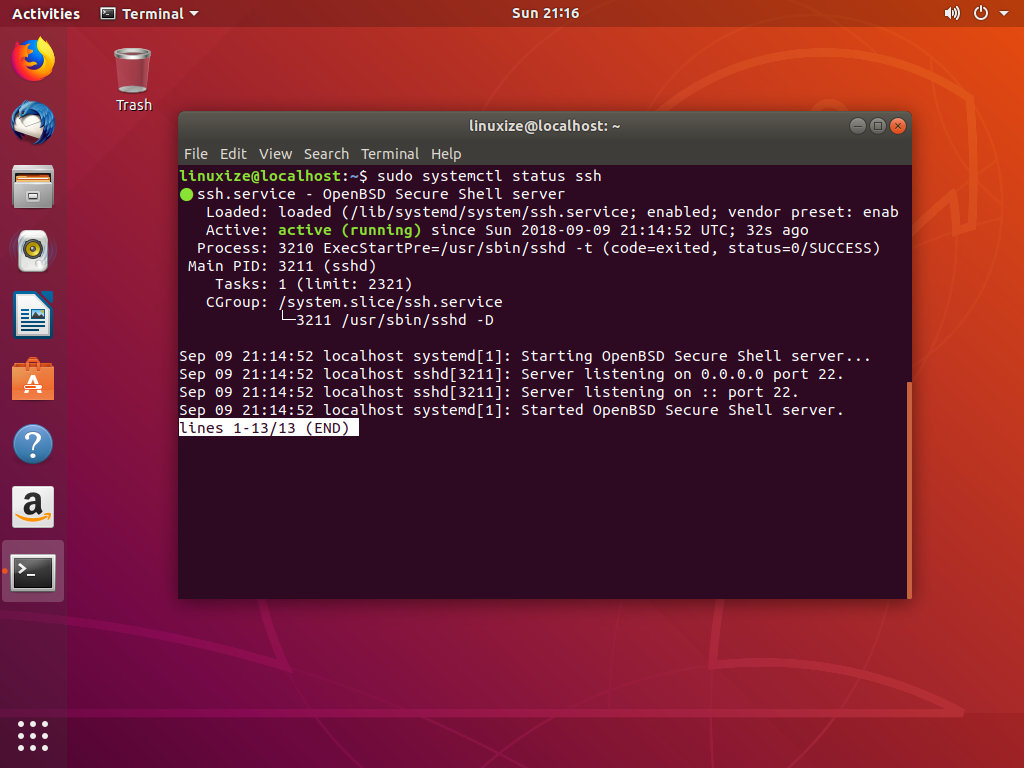
\includegraphics[scale=1]{imagenes/primero/2.png}
    \caption{Servicio de SSH correctamente instalado}
    \label{fig:http1}
\end{figure}
\end{enumerate}
\newpage
\noindent
\subsubsection{Implementación del cliente SSH}
\begin{enumerate}
    \item Se ejecuta el siguiente comando en la terminal\\
    \\sudo apt-get install openssh-client\\
    \\Seguir con los pasos de la instalación
    \item Para conectarse a un servidor SSH se ejecuta la siguiente instrucción\\
    \\ssh -p 22 [username]@[ip]\\
    por ejemplo
    \\ssh -p 22 user{\_}redes@192.168.0.43\\
    \begin{figure}[H]
     \centering
    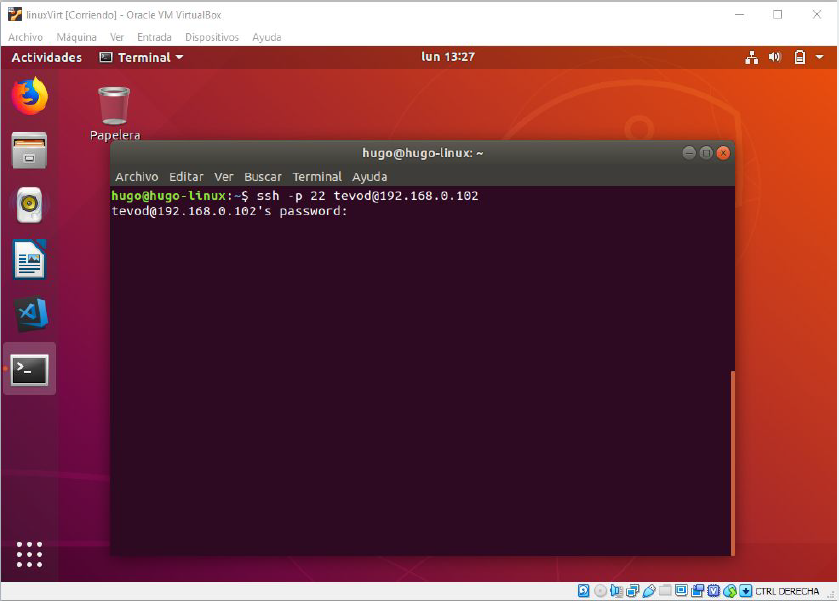
\includegraphics[scale=.54]{imagenes/primero/4.png}
    \caption{Conexión a servidor SSH}
    \label{fig:http1}
\end{figure}
\end{enumerate}
\subsection{Servicio de Nombres de Dominio DNS}
\noindent
Los servidores de DNS traducen los nombres de dominio en una dirección IP y también pueden suceder de manera inversa\\
Para configurar un servicio de DNS en ubuntu se ejecutan los siguientes pasos:
\begin{enumerate}
    \item Se instala el repositorio de bind9
    \\ sudo apt-get install bind9
    \item Nos cambiamos de directorio
    \\ cd /etc/bind/
    \item Editamos el archivo <<named.conf.local>>\\
    agregamos una nueva <<zona>> en la cual va a estar nuestro nombre de dominio agregamos las siguientes lineas al archivo
    \begin{verbatim}
zone "midominio.com"{
    type master;
    file "/etc/bind/db.conf_midominio"
};
\end{verbatim}
El archivo <<db.conf{\_}midominio>> será donde se guarde la ip a resolver
    \item Para crear el archivo <<db.conf{\_}midominio>> tomamos como base el archivo db.local y realizamos una copia\\
    \\sudo cp db.local db.conf{\_}midominio\\
    Remplazamos todos los <<localhost>> por el nombre de nuestro dominio y remplazamos la IP <<127.0.0.1>> por la ip deseada\\
    \begin{verbatim}
BIND    DATA file for local loopback interface;
    $TTL    604800
    @IN     SOA     midominio.com.root.midominio.com(
                                2        ;Serial
                                604800   ;Refresh
                                86400    ;Retry
                                2419200  ;Expire
                                604800 ) ;Negative Cache TTL
        ;
    @       IN      NS      midominio.com.
    @       A       A       192.168.0.43
\end{verbatim}
    \item Reiniciamos el servicio con la siguiente instruccion en la terminal\\
    \\sudo /etc/init.d/bind9 restart\\
    \item Editamos el archivo <<resolv.conf>> para que la computadora utilize el DNS que hemos configurado\\
    \\sudo nano /etc/resolv.conf\\
    Dejamos la siguiente linea en el archivo de texto\\
    \\nameserver 127.0.0.1\\
    \item Probamos el servicio utilizando el siguiente comando\\
    \\host midominio.com\\
    
\clearpage
    \item Para configurar el DNS reverso, es decir dada una ip obtener el nombre de dominio\\
    añadimos otra <<zona>> al archivo de configuracion <<named.conf.local>>\\
    \\sudo nano named.conf.local
     \begin{verbatim}
         ;
            BIND    DATA file for local loopback interface
        ;
        $TTL    604800
        @IN     SOA     midominio.com.root.midominio.com(
                                         2      ;Serial
                                    604800      ;Refresh
                                     86400      ;Retry
                                   2419200      ;Expire
                                    604800 )    ;Negative Cache TTL
        ;
        @       IN      NS      midominio.com.
        34.0.168        IN      PTR     midominio.com.
    \end{verbatim}
    El archivo <<db.192>> contendrá el nombre del dominio el cual va a resolver la ip
    \item Para crear el archivo <<db.192>> nos hacemos una copia del archivo db.127\\
    \\sudo cp db.127 db.192
    \item Remplazamos los <<localhost>> por nuestro dominio y en la ultima linea ingresamos la ip
     \begin{verbatim}
         ;
            BIND    DATA file for local loopback interface
        ;
        $TTL    604800
        @IN     SOA     midominio.com.root.midominio.com(
                                         2      ;Serial
                                    604800      ;Refresh
                                     86400      ;Retry
                                   2419200      ;Expire
                                    604800 )    ;Negative Cache TTL
        ;
        @       IN      NS          midominio.com.
        34.0.168        IN          PTR         midominio.com.
    \end{verbatim}
    \item Reiniciamos el servicio \\
    \\sudo /etc/init.d/bind9 restart\\
    \item Comprobamos que funcione el servicio con el siguiente comando *se ingresa la IP*\\
    \\host 192.168.0.34\\
    
    
\end{enumerate}



\subsection{Servicio de Transferencia de Archivos FTP}
\noindent
El servidor FTP que se configuró fue el de VSFTPD que se encuentra disponible para sistemas UNIX, incluyendo Linux. La configuración de este servidor es simple y ofrece desde los requerimientos mínimos como seguridad, desempeño y estabilidad, hasta requerimientos específicos como la configuración de IPs virtuales, usuarios virtuales, etc.\\    

\noindent
Los pasos que se llevaron a cabo para instalar el servidor FTP y configurarlo fueron los siguientes:

\begin{enumerate}
    \item Ejecutar el siguiente comando en una Terminal de Linux:\\
    
    sudo apt-get install vsftpd\\
    
    En la Figura \ref{fig:ftp1} se puede apreciar la ejecución del comando anterior y su salida.
    
    \begin{figure}[H]
        \centering
        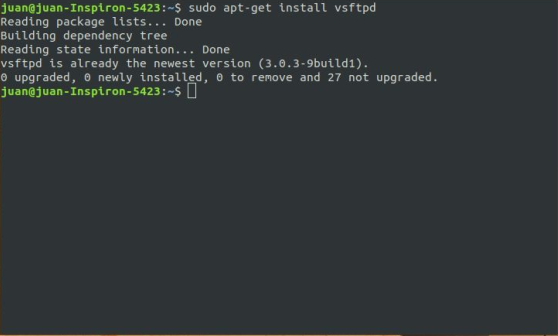
\includegraphics[scale=.97]{imagenes/primero/paso1_ftp.PNG}
        \caption{Instalación del servidor VSFTPD}
        \label{fig:ftp1}
    \end{figure}
    
    \item Verificar la instalación del servidor con el siguiente comando, el cual retorna la versión instalada.\\
    
    vsftpd -version\\
    
    En la Figura \ref{fig:ftp2}, se muestra que se ha instalado correctamente, debido a que el comando retornó la versión correspondiente.

    \begin{figure}[H]
        \centering
        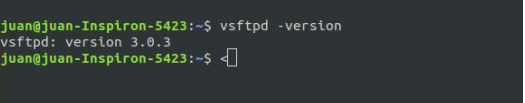
\includegraphics[scale=.97]{imagenes/primero/paso2_ftp.PNG}
        \caption{Verificación de la instalación del servidor VSFTPD}
        \label{fig:ftp2}
    \end{figure}
    
    \item Administrar la ejecución del servidor mediante los siguientes comandos:\\
    
    sudo systemctl restart vsftpd - Reinicia el servidor FTP\\
    
    sudo systemctl start vsftpd - Inicia el servidor FTP\\
    
    sudo systemctl stop vsftpd - Detiene el servidor FTP\\
    
    sudo systemctl stop vsftpd - Detiene el servidor FTP\\
    
    sudo systemctl status vsftpd - Consulta el status del servidor FTP\\
    
    En la Figura \ref{fig:ftp3}, se ejecutan los comandos en un determinado orden para que al ejecutar el que retorna el status del servidor, éste aparezca con el estado de \textbf{active (running)}. 
    
    \begin{figure}[H]
        \centering
        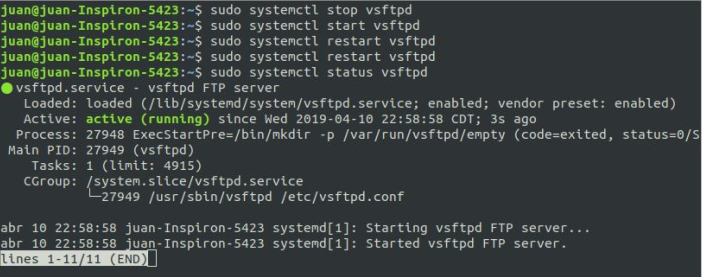
\includegraphics[scale=.80]{imagenes/primero/paso3_ftp.PNG}
        \caption{Administración de la ejecución}
        \label{fig:ftp3}
    \end{figure}
    
    \item Verificar el estado del firewall. Es necesario permitir las conexiones a los puertos 20 y 21. En algunas distribuciones UNIX el firewall bloquea estos puertos. Así, lo anterior se puede llevar a cabo con los siguientes comandos:\\
    
    sudo ufw status\\
    
    sudo ufw allow 21\\
    
    sudo ufw allow 21\\
    
    En la Figura \ref{fig:ftp4}, se puede apreciar la ejecución de los comandos anteriores.
    
    \begin{figure}[H]
        \centering
        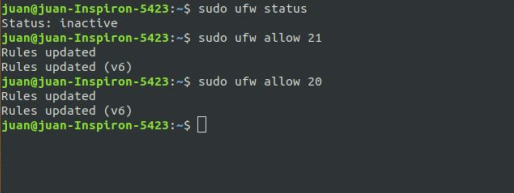
\includegraphics[scale=1.05]{imagenes/primero/paso4_ftp.PNG}
        \caption{Verificar estado de firewall y permitir el uso de los puertos 20 y 21}
        \label{fig:ftp4}
    \end{figure}
\end{enumerate}

\noindent
Como cliente FTP, es posible conectarse al servidor mediante un navegador o usando Filezilla, el cual es un cliente que soporta los protocolos FTP, SFTP y FTPS.

\noindent
En este caso se utilizó un navegador web. Para esto es necesario ingresar la siguiente línea en la barra de direcciones del navegador:\\

\noindent
ftp://url\\

\noindent
Donde url es la IP del servidor o bien puede ser localhost en el caso en el que se estén realizando pruebas de manera local.\\

\noindent
En la Figura \ref{fig:ftp5}, se puede apreciar la ejecución de los comandos anteriores.
    
\begin{figure}[H]
    \centering
    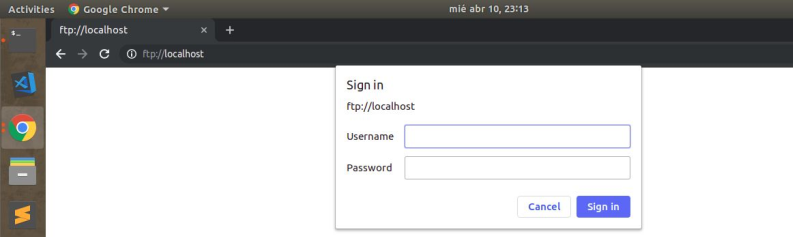
\includegraphics[scale=.75]{imagenes/primero/cliente_ftp.PNG}
    \caption{Accediendo a los recursos de VSFTPD mediante un navegador web}
    \label{fig:ftp5}
\end{figure}

\noindent
Por default, el usuario y la contraseña son \textbf{root}, por lo cual se recomienda crear un nuevo usuario que tenga únicamente los permisos necesarios.\\

\noindent
La Figura \ref{fig:ftp6}, muestra el árbol de directorios a los que se pueden acceder.

\begin{figure}[H]
    \centering
    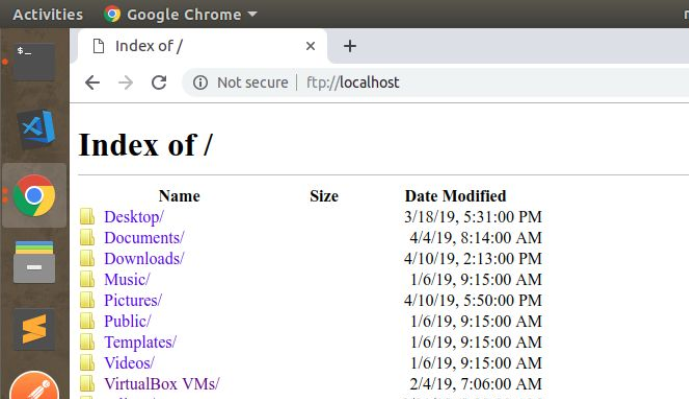
\includegraphics[scale=.75]{imagenes/primero/cliente_ftp2.PNG}
    \caption{Directorios disponibles}
    \label{fig:ftp6}
\end{figure}

\noindent
Si se desea descargar algún recurso, basta con dar click encima del mismo para que se comience la descarga.\\

\noindent
La Figura \ref{fig:ftp7}, corresponde a la evidencia que fue adjuntada para la evaluación para validar que el servidor de FTP que se configuró funciona correctamente.

\begin{figure}[H]
    \centering
    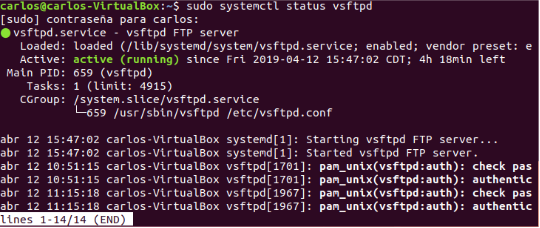
\includegraphics[scale=.75]{imagenes/primero/servidor_ftp.PNG}
    \caption{Comando sudo systemctl status vsftpd para visualizar el status del servidor FTP}
    \label{fig:ftp7}
\end{figure}

\subsection{Servicio de correo electrónico SMTP}
\noindent
Para la transferencia de datos que componen a los correos electrónicos se utiliza el protocolo SMTP, que define una serie de normas para el envío. Para ello este servicio utiliza una estructura cliente-servidor.\\

\noindent
Para instalar y configurar el servicio de correo electrónico usando SMTP en Ubuntu es necesario Postfix, el cual, es un agente de transporte de correo de manera que nos permite enrutar y
transferir correos electrónicos. Así, se llevaron a cabo los siguientes pasos:

\begin{enumerate}
    \item Ejecutar el siguiente comando para instalar Postfix:\\
    
    sudo apt-get install postfix\\
    
    \item En la configuración de Postfix se elige “Sitio de internet”\\
    
    En la Figura \ref{fig:smtp1}, se muestran las opciones disponibles para la configuración de Postfix.
    
    \begin{figure}[H]
        \centering
        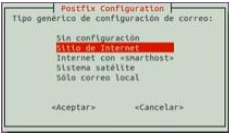
\includegraphics[scale=1.5]{imagenes/primero/paso2_smtp.PNG}
        \caption{Configuración de Postfix}
        \label{fig:smtp1}
    \end{figure}
    
    \item Se escribe el dominio “redes.com”, el cual será el nombre del host
    
    \noindent
    En la Figura \ref{fig:smtp2}, se puede apreciar que la configuración solicita que se ingrese el nombre del sistema del correo; es decir, del host.
    
    \begin{figure}[H]
        \centering
        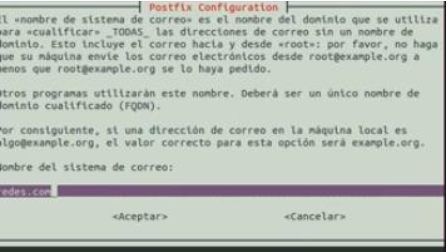
\includegraphics[scale=1.2]{imagenes/primero/paso3_smtp.PNG}
        \caption{Asignando nombre al sistema de correo}
        \label{fig:smtp2}
    \end{figure}
    
    \item Para hacer cambios en la configuración de Postfix tenemos que editar el archivo “etc/postfix/main.cf”. Después de modificar dicho archivo, debemos asegurarnos de ejecutar “etc/init.d/postfix reload” o el comando “service postfix restart” para que los cambios sean aplicados. Para modificar el archivo, usamos “nano /etc/postfix/main.cf” con la finalidad de poder configurar la dirección IP\\
    
    En la Figura \ref{fig:smtp3}, se puede observar el parte del contenido del archivo main.cf. Para configurar la dirección IP, en la Figura \ref{fig:smtp4}, se muestra cómo debe de quedar configurada.
    
    \begin{figure}[H]
        \centering
        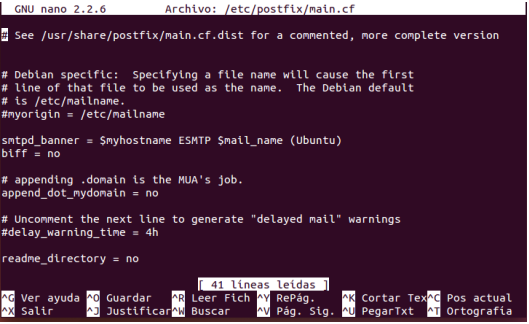
\includegraphics[scale=1.05]{imagenes/primero/paso4_1_smtp.PNG}
        \caption{Parte del contenido del archivo main.cf}
        \label{fig:smtp3}
    \end{figure}
    
    \begin{figure}[H]
        \centering
        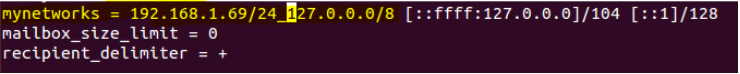
\includegraphics[scale=.75]{imagenes/primero/paso4_2_smtp.PNG}
        \caption{Configuración de la dirección IP}
        \label{fig:smtp4}
    \end{figure}
    
    \item Se reinicia el servicio de Postfix para que los cambios surtan efecto.\\
    
    \noindent
    En la Figura \ref{fig:smtp5}, se tiene la salida del comando "sudo service postfix restart".

    \begin{figure}[H]
        \centering
        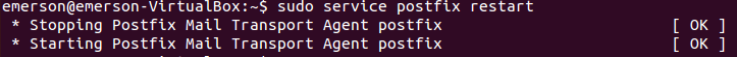
\includegraphics[scale=.75]{imagenes/primero/paso5_smtp.PNG}
        \caption{Reinicio del servicio Postfix}
        \label{fig:smtp5}
    \end{figure}
    
    \item Es necesario instalar el paquete “mailutils” para enviar correos desde la línea de comandos. Nota: se puede usar mailx. Por lo tanto, se ejecuta el comando “sudo aptget install mailutils"
    
    En la Figura \ref{fig:smtp6}, se tiene la salida del comando "sudo aptget install mailutils".
    
    \begin{figure}[H]
        \centering
        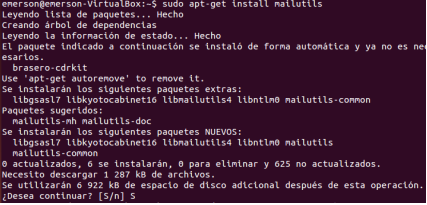
\includegraphics[scale=1.3]{imagenes/primero/paso6_smtp.PNG}
        \caption{Instalación de mailutils}
        \label{fig:smtp6}
    \end{figure}
    
    \item Creación de usuarios para realizar pruebas del correcto funcionamiento del servidor. Para esto, es necesario utilizar los comandos que ofrece mailutils.\\
    
    \noindent
    Por ejemplo, para enviar un correo a user@example.com, se ejecuta la siguiente línea en una Terminal:\\
    
    \noindent
    mail user@example.com\\
    
    \noindent
    La cual va a devolver como salida lo siguiente:\\
    
    \noindent
    Cc:\\
    \noindent
    Subject:\\
    
    \noindent
    En “Cc:” se pone un destinatario que recibirá una copia del correo. En “Subject:” el asunto del mensaje. Después, se podrá escribir libremente el contenido del mensaje y para terminar de redactar el contenido se pulsa CONTRL-D para finalizar y enviar el mensaje.
    
    \item Ejecución del comando “adduser nombre\_usuario” para agregar un usuario al servidor de correo. Nota: para ello es necesario agregarlo como super usuario con sudo su antecediendo el comando anterior.\\
    
     En la Figura \ref{fig:smtp7}, se tiene la salida del comando ``adduser nombre\_usuario''.
    
    \begin{figure}[H]
        \centering
        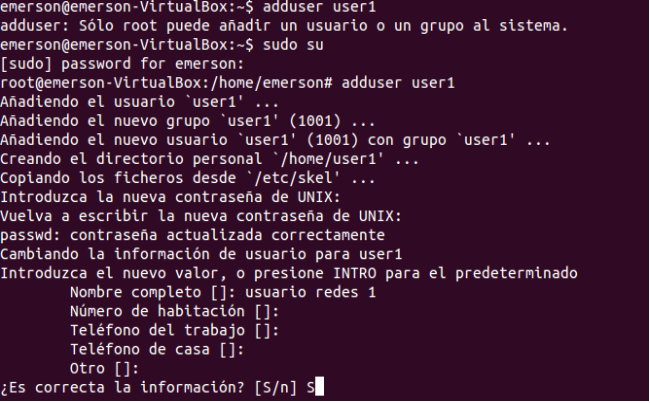
\includegraphics[scale=.85]{imagenes/primero/paso7_smtp.PNG}
        \caption{Creación de usuarios del servidor de correo}
        \label{fig:smtp7}
    \end{figure}
    
    \item Inicio de sesión de alguno de los usuarios creados. Esta acción se puede apreciar en la Figura \ref{fig:smtp8}
    
    \begin{figure}[H]
        \centering
        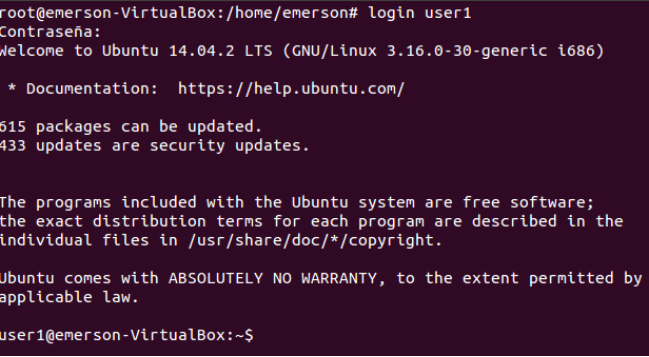
\includegraphics[scale=.85]{imagenes/primero/paso8_smtp.PNG}
        \caption{Inicio de sesión}
        \label{fig:smtp8}
    \end{figure}
    
    \item Envío de correo a un usuario diferente usando ``mail nombre\_usuario@host''. Se termina de redactar con Ctrl+D. Veáse la Figura \ref{fig:smtp9}
    
    \begin{figure}[H]
        \centering
        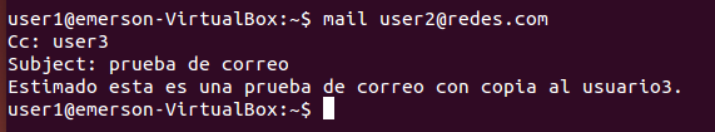
\includegraphics[scale=.77]{imagenes/primero/paso9_smtp.PNG}
        \caption{Envío de correo}
        \label{fig:smtp9}
    \end{figure}
    
    \item Cierre de sesión utilizando “logout” para iniciar sesión con el usuario a quien se le mando el correo. Se puede observar en la Figura \ref{fig:smtp10} que en primera instancia aparece el mensaje ``tiene correo''
    
    \begin{figure}[H]
        \centering
        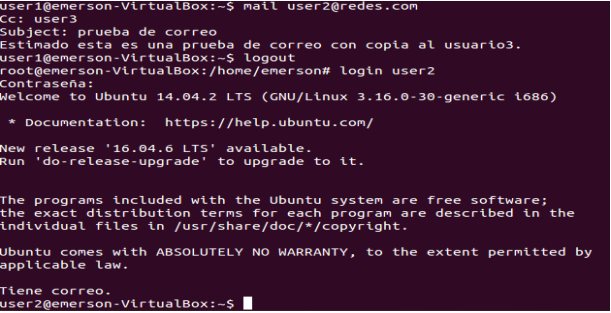
\includegraphics[scale=.77]{imagenes/primero/paso10_smtp.PNG}
        \caption{Consultando bandeja de entrada}
        \label{fig:smtp10}
    \end{figure}
    
    \item Con el comando “mail” se ve el correo que está en bandeja de entrada y se selecciona el correo con el número que le corresponde. Veáse la Figura \ref{fig:smtp11}
    
    \begin{figure}[H]
        \centering
        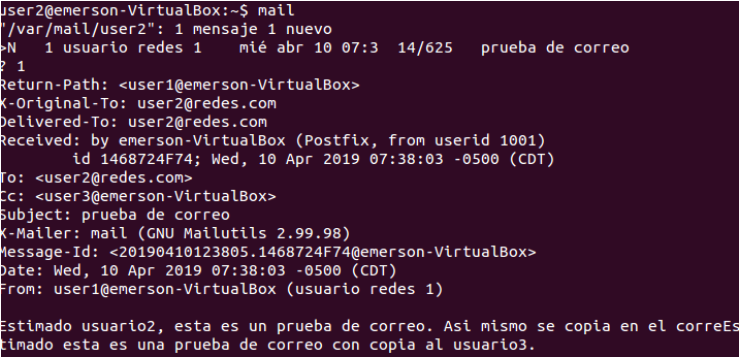
\includegraphics[scale=.75]{imagenes/primero/paso11_smtp.PNG}
        \caption{Visualizando correo recibido}
        \label{fig:smtp11}
    \end{figure}
    
    \item Instalación de dovecot, el cual permitirá ver los correos en un MDA, para ello dovecot usa los protocolos pop e imap. Para realizar esto, se debe ejecutar el siguiente comando:\\
    
    sudo apt-get install dovecot-po3d dovecotimapd\\
    
    \noindent
    En la Figura \ref{fig:smtp12}, se muestra la salida del comando anterior.
    
    \begin{figure}[H]
        \centering
        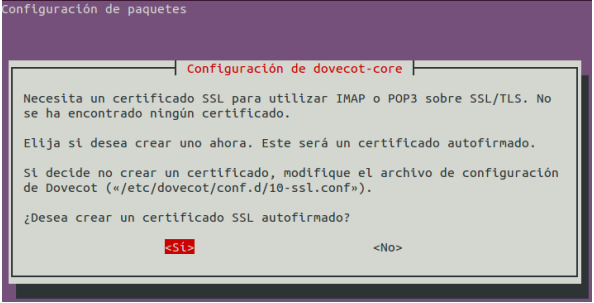
\includegraphics[scale=.95]{imagenes/primero/paso12_smtp.PNG}
        \caption{Instalación de Dovecot}
        \label{fig:smtp12}
    \end{figure}
    
    En el nombre del equipo, para este caso, se escribirá ``redes.com''.
    
    \item Modificación del archivo de configuración con “sudo nano /etc/dovecot/dovecot.conf” para quitar el comentario “listen”. Esta acción se muestra en la Figura \ref{fig:smtp13}
    
    \begin{figure}[H]
        \centering
        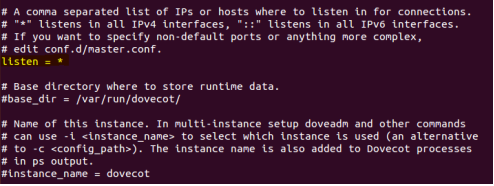
\includegraphics[scale=1.13]{imagenes/primero/paso13_smtp.PNG}
        \caption{Modificación del archivo dovecot.conf}
        \label{fig:smtp13}
    \end{figure}
    
    \item Se ubica el fichero de configuración donde se asegura que sea una conexión segura. Para ello, es necesario ejecutar el siguiente comando: ``sudo nano /etc/dovecot/conf.d/10-auth.conf''. Veáse la Figura \ref{fig:smtp14}
    
    \begin{figure}[H]
        \centering
        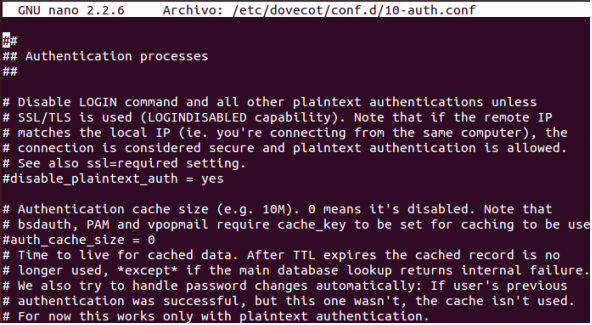
\includegraphics[scale=.95]{imagenes/primero/paso14_smtp.PNG}
        \caption{Modificación del archivo 10-auth.conf}
        \label{fig:smtp14}
    \end{figure}
    
    \noindent
    Posteriormente, se elimina el comentario a la directriz ``diseable\_plaintext\_auth'' y se agrega el valor ``no''. De tal forma que quede ``diseable\_plaintext\_auth=no''.\\
    
    \item Se abre el archivo ``sudo nano /etc/dovecot/conf.d/10-mail.conf'' para la ubicación del mail. Esta acción se puede visualizar en la Figura \ref{fig:smtp15}
    
    \begin{figure}[H]
        \centering
        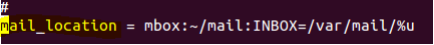
\includegraphics[scale=1]{imagenes/primero/paso15_smtp.PNG}
        \caption{Ubicación del mail}
        \label{fig:smtp15}
    \end{figure}
    
    \item Se reinicia el servicio con ``service dovecot restart'' (Figura \ref{fig:smtp16})
    
    \begin{figure}[H]
        \centering
        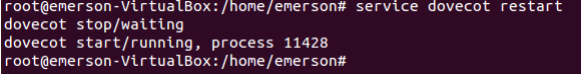
\includegraphics[scale=.96]{imagenes/primero/paso16_smtp.PNG}
        \caption{Reinicio del servicio}
        \label{fig:smtp16}
    \end{figure}
    
    \item Verificar que el servidor tenga montado imap y pop3. Veáse la Figura \ref{fig:smtp17}
    
    \begin{figure}[H]
        \centering
        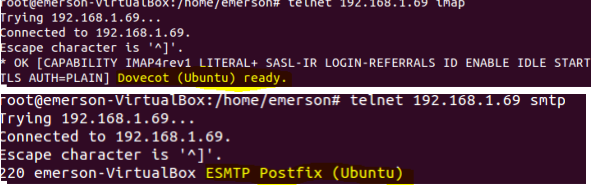
\includegraphics[scale=.96]{imagenes/primero/paso17_smtp.PNG}
        \caption{Verifiación de componentes instalados}
        \label{fig:smtp17}
    \end{figure}
    
    \item Agregamos en los hosts la dirección y dominio del servidor (/etc/hosts) con el comando ``sudo nano /etc/hosts'' (Figura \ref{fig:smtp18})
    
    \begin{figure}[H]
        \centering
        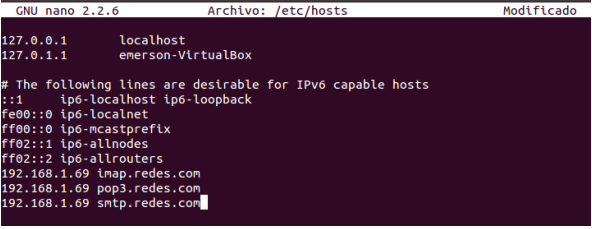
\includegraphics[scale=.96]{imagenes/primero/paso18_smtp.PNG}
        \caption{Modificación del archivo hosts}
        \label{fig:smtp18}
    \end{figure}
    
    \item Se eliminan los comentarios para las líneas ``ssl=yes , ssl\_cent\_file y ssl\_key'' (Figura \ref{fig:smtp19})
    
    \begin{figure}[H]
        \centering
        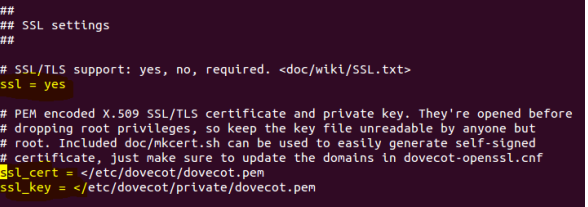
\includegraphics[scale=.95]{imagenes/primero/paso19_smtp.PNG}
        \caption{Eliminación de comentarios en las líneas de ssl}
        \label{fig:smtp19}
    \end{figure}
    
    \item Se abre fichero de configuración de Postfix con ``sudo nano /etc/postfix/master.cf'' (Figura \ref{fig:smtp20})
    
    \begin{figure}[H]
        \centering
        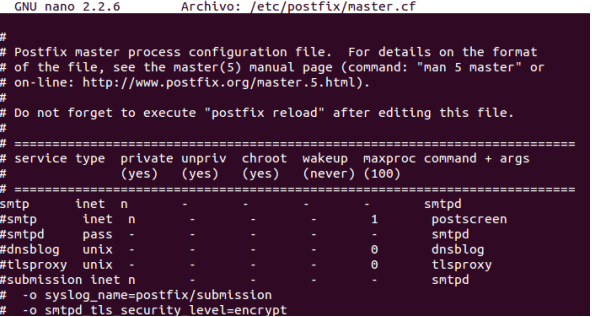
\includegraphics[scale=.95]{imagenes/primero/paso20_smtp.PNG}
        \caption{Visualización de archivo master.cf}
        \label{fig:smtp20}
    \end{figure}
    
    \noindent
    Se eliminan los comentarios a las líneas sombreadas en la Figura \ref{fig:smtp21}
    
    \begin{figure}[H]
        \centering
        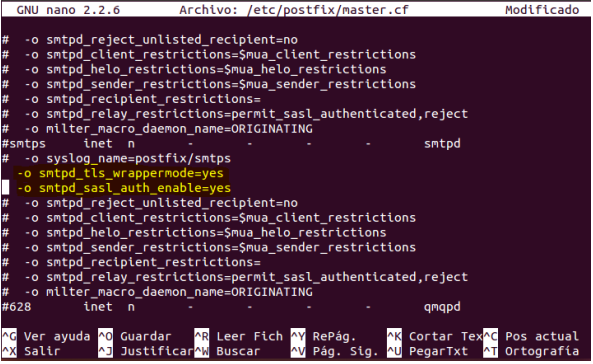
\includegraphics[scale=.95]{imagenes/primero/paso21_smtp.PNG}
        \caption{Eliminación de comentarios}
        \label{fig:smtp21}
    \end{figure}
    
    \item Se reinicia el servicio de Postfix (Figura \ref{fig:smtp22})
    
    \begin{figure}[H]
        \centering
        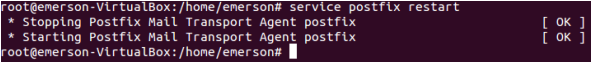
\includegraphics[scale=.95]{imagenes/primero/paso22_smtp.PNG}
        \caption{Reinicio del servicio Postfix}
        \label{fig:smtp22}
    \end{figure}
    
    \item Hasta este punto se configuró e instaló correctamente postfix, y dovecot. Además, se probó el funcionamiento correcto del servidor y apartir de este punto se puede usar Thunderbird el cual es un cliente de correo electrónico open/source.
\end{enumerate}

\noindent
Las Figuras que se muestran a continuación, servieron de ayuda para utilizar Thunderbird.

\begin{figure}[H]
    \centering
    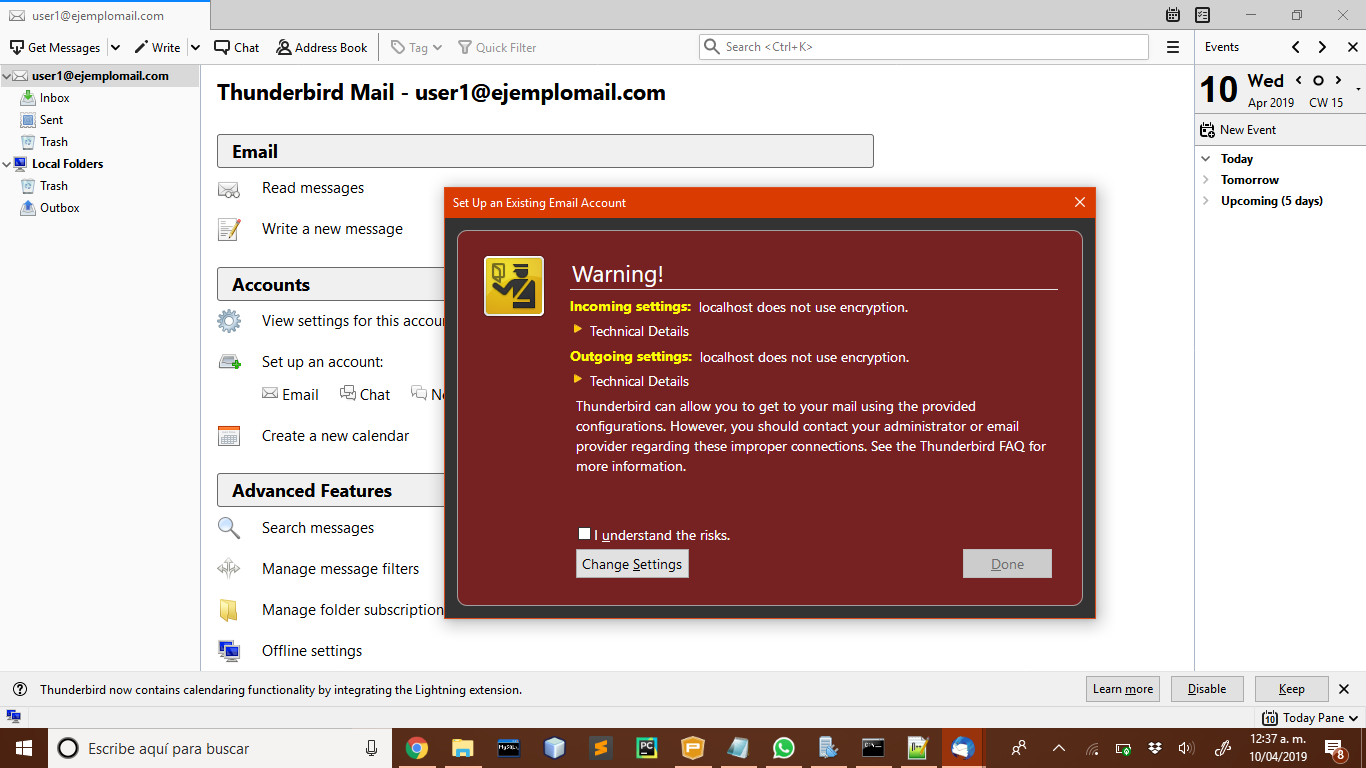
\includegraphics[scale=.30]{imagenes/primero/AceptarRiesgo.png}
    \caption{Se acepta el riesgo}
    \label{fig:smtp23}
\end{figure}

\begin{figure}[H]
    \centering
    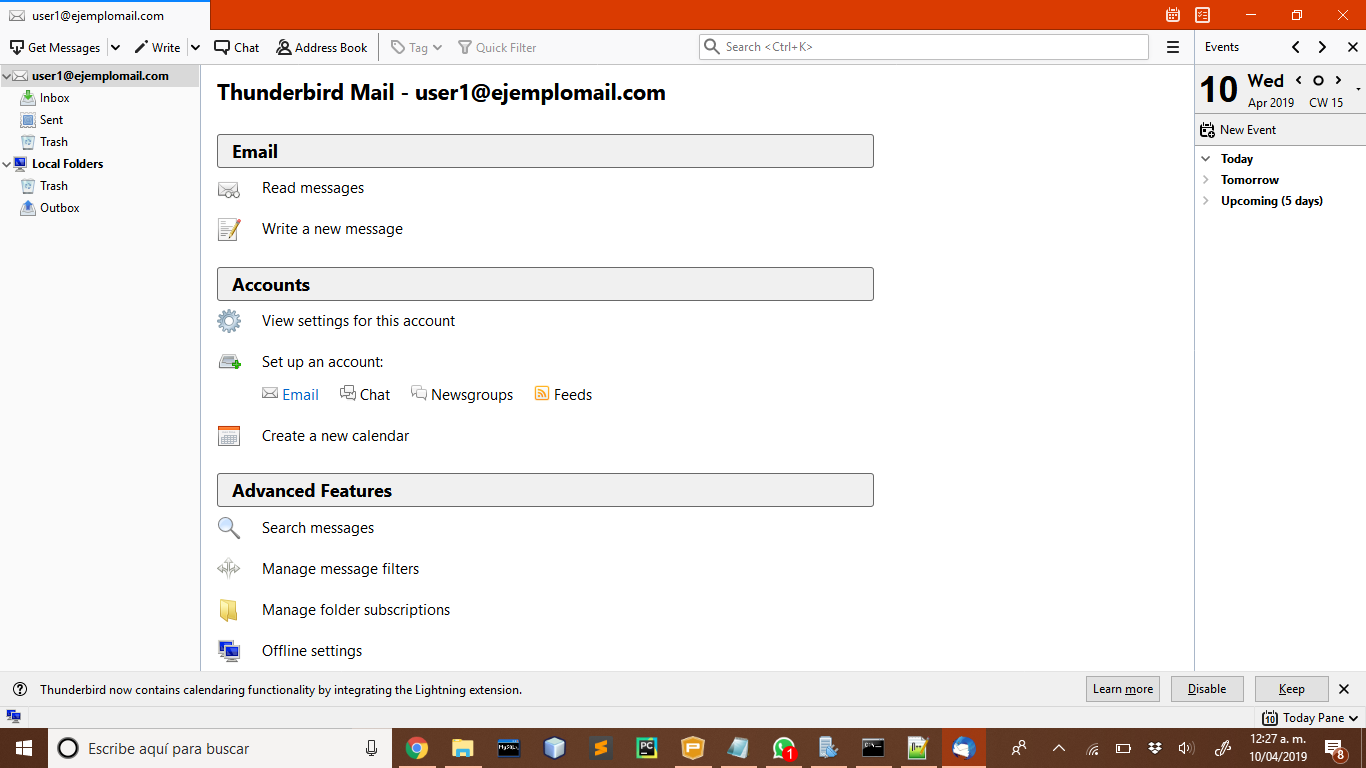
\includegraphics[scale=.30]{imagenes/primero/InicioThunderbird.png}
    \caption{Inicio de Thunderbird}
    \label{fig:smtp24}
\end{figure}

\begin{figure}[H]
    \centering
    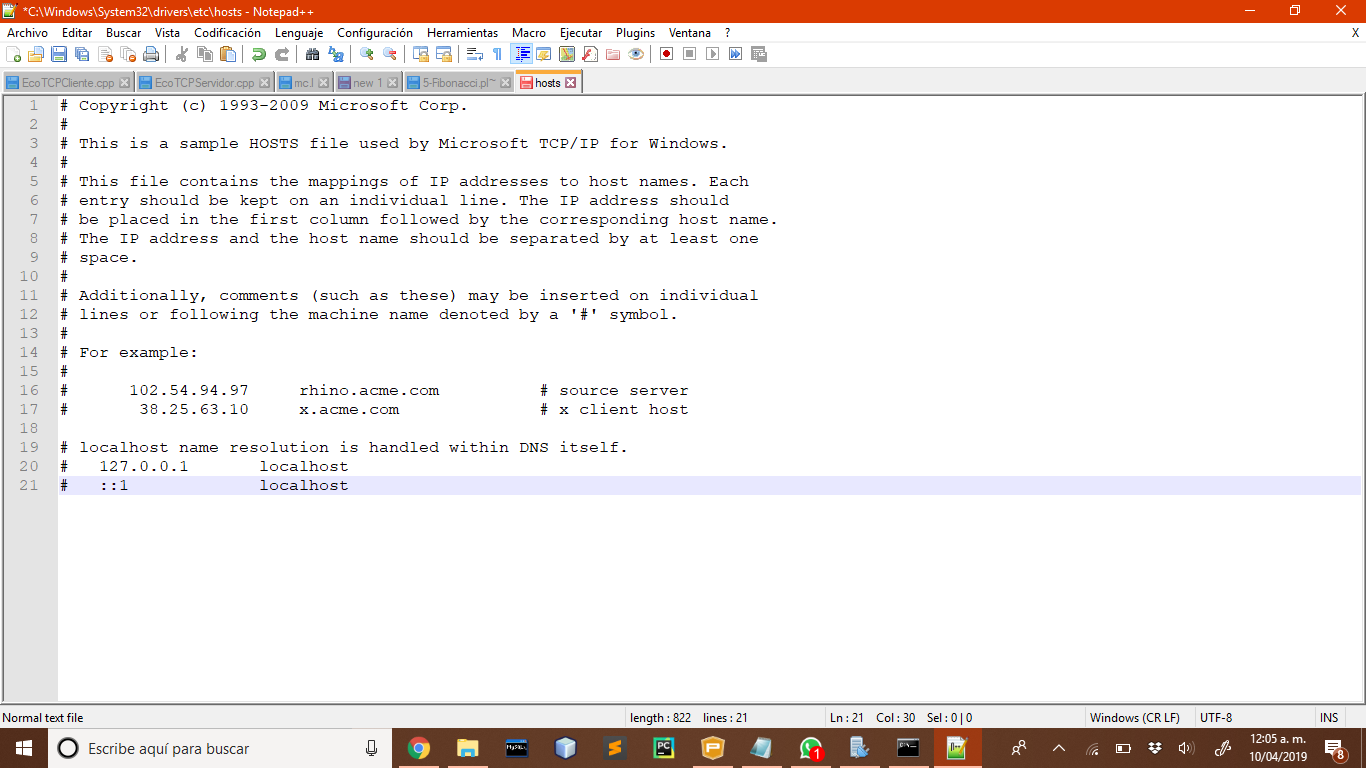
\includegraphics[scale=.30]{imagenes/primero/AgregarIP.png}
    \caption{Se agrega la IP en el archivo Hosts}
    \label{fig:smtp25}
\end{figure}

\begin{figure}[H]
    \centering
    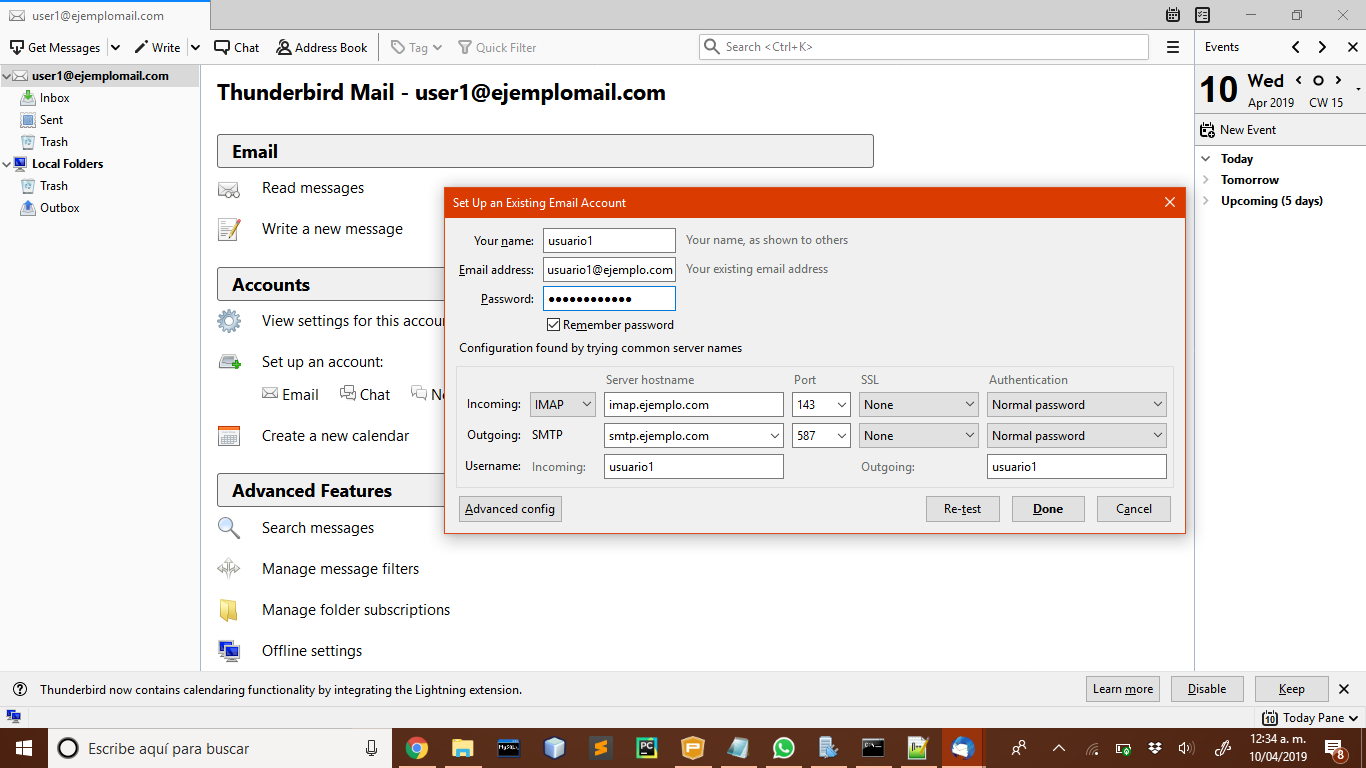
\includegraphics[scale=.30]{imagenes/primero/ConfiguracionInicio.png}
    \caption{Configuración del inicio}
    \label{fig:smtp26}
\end{figure}

\begin{figure}[H]
    \centering
    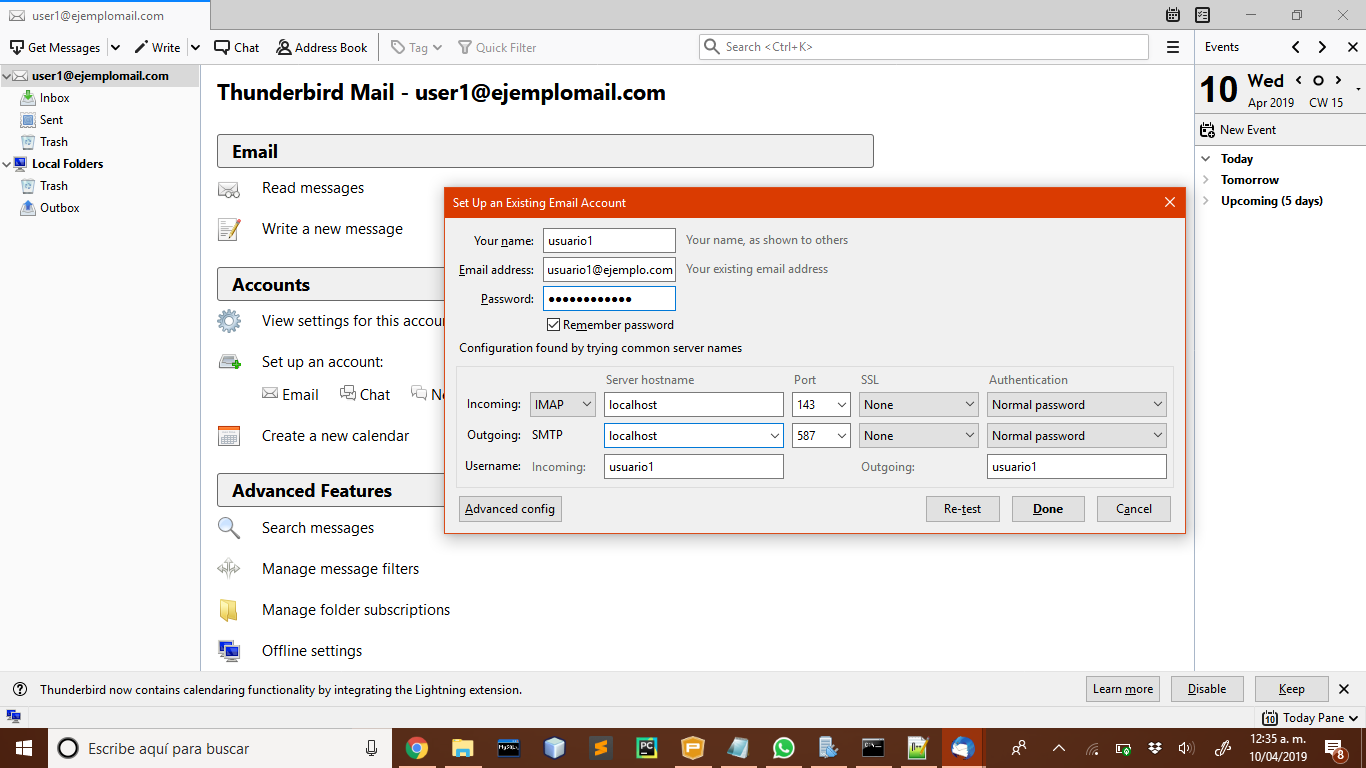
\includegraphics[scale=.30]{imagenes/primero/RegistroThunderbird.png}
    \caption{Registro}
    \label{fig:smtp27}
\end{figure}

\begin{figure}[H]
    \centering
    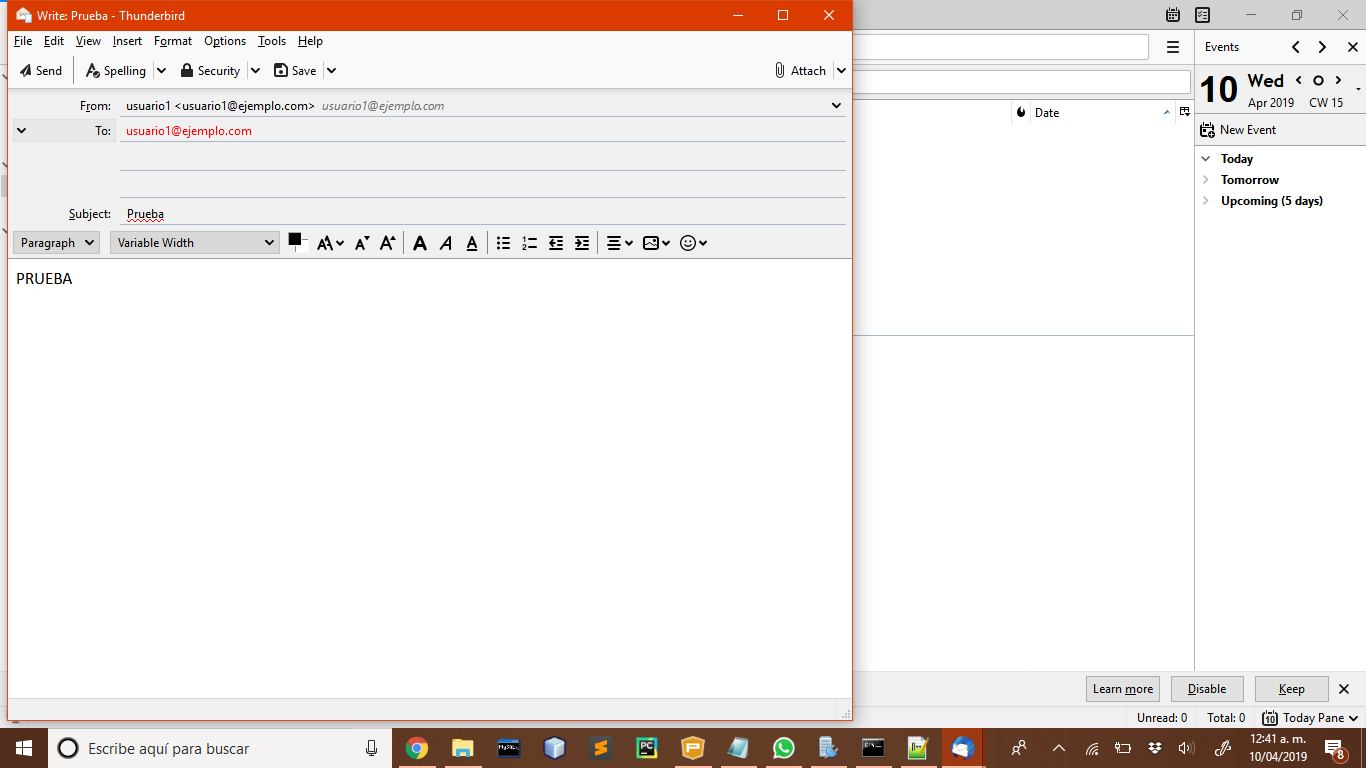
\includegraphics[scale=.30]{imagenes/primero/EnviarCorreo.png}
    \caption{Enviar correo}
    \label{fig:smtp28}
\end{figure}

\noindent
Las Figuras siguientes, corresponden a la evidencia que fue adjuntada para la evaluación para validar que el servidor de correo que se configuró funciona correctamente.

\begin{figure}[H]
    \centering
    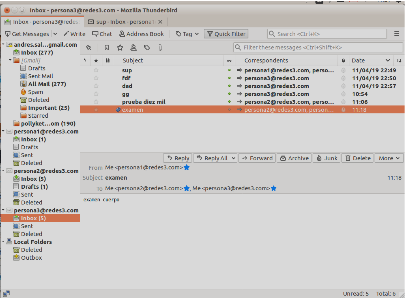
\includegraphics[scale=1.20]{imagenes/primero/evidencia1_smtp.PNG}
    \caption{Mensaje enviado a persona 3 desde persona 1}
    \label{fig:smtp29}
\end{figure}

\begin{figure}[H]
    \centering
    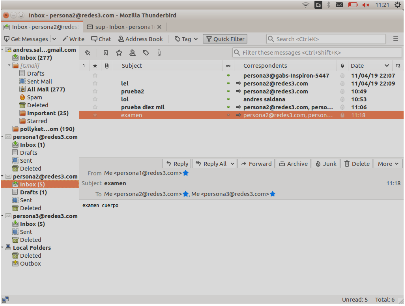
\includegraphics[scale=1.20]{imagenes/primero/evidencia2_smtp.PNG}
    \caption{Mensaje enviado a persona 2 desde persona 1}
    \label{fig:smtp30}
\end{figure}

\begin{figure}[H]
    \centering
    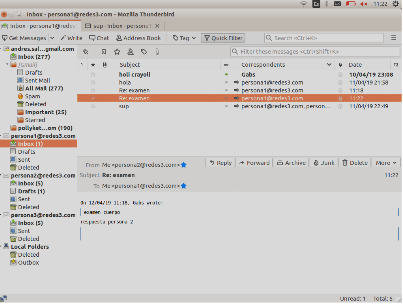
\includegraphics[scale=1.20]{imagenes/primero/evidencia3_smtp.PNG}
    \caption{Mensaje respondido a persona 1 desde persona 2}
    \label{fig:smtp31}
\end{figure}

\begin{figure}[H]
    \centering
    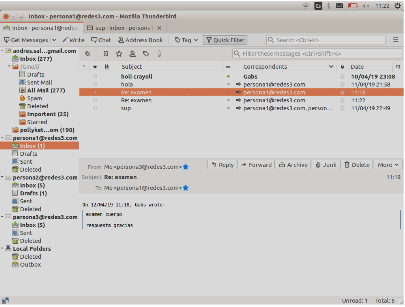
\includegraphics[scale=1.20]{imagenes/primero/evidencia4_smtp.PNG}
    \caption{Mensaje respondido a persona 1 desde persona 3}
    \label{fig:smtp32}
\end{figure}